\documentclass{beamer}
\usepackage{ragged2e}
\usepackage{amsmath,amssymb}

\title{Modelos Generativos Profundos}
\subtitle{Clase 11: Redes generativas adversarias (parte II)}
\author{Fernando Fêtis Riquelme}
\institute{
    Facultad de Ciencias Físicas y Matemáticas\\
    Universidad de Chile
}
\date{Primavera, 2025}
\titlegraphic{\hfill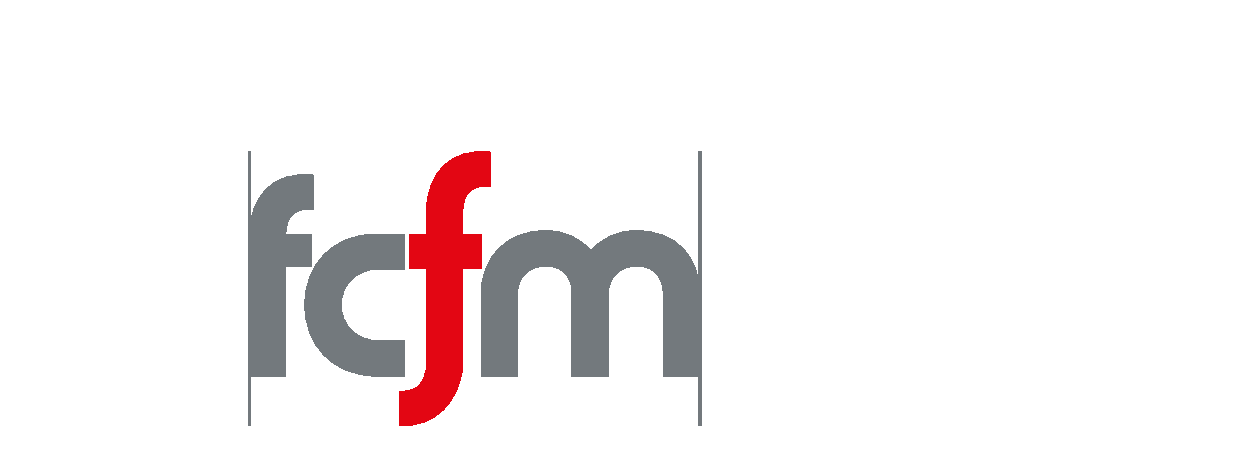
\includegraphics[height=1.2cm]{images/fcfm}}

\usetheme{metropolis}
\setbeamercovered{transparent}

\newcommand{\R}{\mathbb{R}}
\newcommand{\N}{\mathbb{N}}
\newcommand{\Z}{\mathbb{Z}}
\newcommand{\argmax}{\operatorname{argmax}}
\newcommand{\insertimage}[2]{
    \begin{center}
        \includegraphics[width=#2\textwidth]{images/#1}
    \end{center}
}
\setlength{\leftmargini}{0em}
\renewcommand{\raggedright}{\leftskip=0pt \rightskip=0pt plus 0cm}

\justifying

\begin{document}

\begin{frame}
    \titlepage
\end{frame}

\begin{frame}{Clase de hoy}
    \tableofcontents
\end{frame}

\section{Redes convolucionales y convolución transpuesta}

\begin{frame}{Redes neuronales convolucionales}
    Si se utilizan redes MLP para procesar imágenes, entonces cada pixel de la imagen se relaciona del mismo modo con todos los otros pixeles, por lo que no se aprovecha la estructura espacial 2D de las imágenes. Las \textbf{redes neuronales convolucionales (CNNs)} utilizan \textbf{filtros convolucionales}, lo que induce:
    \begin{itemize}
        \item \textbf{Sesgo de localidad}: cada neurona solo ve una vecindad local de la entrada (campo receptivo).
        \item \textbf{Equivarianza traslacional}: un filtro convolucional detecta el mismo patrón sin importar dónde se encuentre en la imagen.
    \end{itemize}
    Recordar que, usualmente, las CNNs van reduciendo la resolución de los mapas de características al mismo tiempo que aumentan la cantidad de canales.
\end{frame}

\begin{frame}{Redes neuronales convolucionales}
    En IA generativa, es usual generar una imagen aumentando progresivamente la resolución de una representación latente inicial. Para esto, se pueden usar dos enfoques:
    \begin{itemize}
        \item Upsampling por interpolación.
        \item Convolución transpuesta.
    \end{itemize}
    \insertimage{interpolation}{0.6}
\end{frame}

\begin{frame}{Operación convolución y convolución transpuesta}
    Para entender mejor el operador convolución (más correctamente, cross-correlation), se tiene el siguiente ejemplo de una convolución 1D para un filtro $K=[5, 10, 15, 20]$:

    Dada una entrada $x=(1,2,3,4,5,6,7,8,9,10)^\top\in\R^{10}$, la salida de la convolución (asumiendo $\text{stride}=2$ y $\text{padding}=0$) es el vector $y\in\R^4$  cuyas coordenadas son
    \begin{align*}
         & y_1=5\cdot1 + 10\cdot2 + 15\cdot3 +20\cdot4  =150 \\
         & y_2=5\cdot3 + 10\cdot4 + 15\cdot5 +20\cdot6  =250 \\
         & y_3=5\cdot5 + 10\cdot6 + 15\cdot7 +20\cdot8  =350 \\
         & y_4=5\cdot7 + 10\cdot8 + 15\cdot9 +20\cdot10 =450 \\
    \end{align*}
\end{frame}

\begin{frame}{Operación convolución y convolución transpuesta}
    La convolución es una \textbf{transformación lineal}, por lo que puede representarse como una multiplicación matricial de la forma $x\mapsto Wx$, donde $W$ es una matriz que depende del filtro convolucional (y de otros parámetros como el stride y padding).

    En particular, para el ejemplo anterior, se tiene que $y=Wx$, donde $W\in\mathcal{M}_{4,10}(\R)$ es la \textbf{matriz de Toeplitz} definida como
    \begin{equation*}
        W=\begin{pmatrix}
            5 & 10 & 15 & 20 & 0  & 0  & 0  & 0  & 0  & 0  \\
            0 & 0  & 5  & 10 & 15 & 20 & 0  & 0  & 0  & 0  \\
            0 & 0  & 0  & 0  & 5  & 10 & 15 & 20 & 0  & 0  \\
            0 & 0  & 0  & 0  & 0  & 0  & 5  & 10 & 15 & 20 \\
        \end{pmatrix}
    \end{equation*}
    En convoluciones 2D también es posible hacer esto. En estos casos, la matriz $W$ tiene una estructura más compleja, pero sigue siendo posible definirla.
\end{frame}

\begin{frame}{Operación convolución y convolución transpuesta}
    Dada una convolución representada por $x\in\R^n\mapsto Wx\in\R^m$ (con $W\in\mathcal{M}_{m,n}(\R)$), la \textbf{convolución transpuesta} es el operador asociado a la transformación lineal $x\in\R^m\mapsto W^Tx\in\R^n$.

    Si la convolución reduce la dimensión de la entrada, la convolución transpuesta la aumenta, por lo que esta operación puede interpretarse como una especie de \textit{convolución inversa}. 

    En el ejemplo anterior, la convolución mapeaba vectores de $\R^{10}$ a vectores de $\R^4$, mientras que la convolución transpuesta mapea vectores $x\in\R^4$ a vectores de $y\in\R^{10}$.

    Esto se extiende naturalmente a convoluciones 2D. En consecuencia, la convolución transpuesta permite aumentar la resolución espacial de los mapas de características en una CNN.
\end{frame}

\section{DCGAN y U-Net para segmentación}

\begin{frame}{DCGAN}
    La naturaleza adversativa de una GAN provoca que su entrenamiento sea muy inestable. El trabajo de \textbf{deep convolutional GAN (DCGAN)} entrega algunas heurísticas para usar CNNs en el generador y en el discriminador de una GAN:
    \begin{itemize}
        \item El discriminador es una CNN clásica (sin convoluciones transpuestas) y el generador es una CNN transpuesta.
        \item Usar BatchNorm en todas las capas del generador y discriminador, excepto en la capa de entrada del discriminador y la capa de salida del generador.
        \item Usar ReLU en todas las capas del generador, excepto en la salida donde se recomienda utilizar $\tanh$. Pero usar LeakyReLU en todas las capas del discriminador.
        \item etc.
    \end{itemize}
\end{frame}

\begin{frame}{DCGAN}
    DCGAN también estudia la estructura algebraica que emerge en el espacio latente de la GAN: ciertas operaciones vectoriales sobre representaciones latentes se traducen en transformaciones coherentes en el espacio de las imágenes generadas.

    Un ejemplo es la \textbf{interpolación semántica}. Si $z_0,z_1\in\R^L$ son dos muestras de la variable latente $p(z)\sim\mathcal{N}(0,\text{I}_L)$, entonces es posible construir una interpolación latente entre las muestras $G_\theta(z_0),G_\theta(z_1)\in\R^D$ considerando $x_t=G_\theta((1-t)z_0+tz_1)\in\R^D$, donde $t\in[0,1]$ es un parámetro de interpolación.
    \insertimage{dcgan_interpolation}{0.7}
\end{frame}

\begin{frame}{DCGAN}
    La estructura vectorial del espacio latente $\R^L$ también permite hacer otro tipo de operaciones. Para esto, considerar:
    \begin{itemize}
        \item $z_\text{man, glasses}\in\R^L$ es un promedio de vectores latentes que generan hombres con lentes.
        \item $z_\text{man, no glasses}\in\R^L$ es lo mismo pero genera hombres sin lentes.
        \item  $z_\text{woman, no glasses}\in\R^L$ es lo mismo pero genera mujeres sin lentes.
    \end{itemize}
    entonces el vector latente (e incluso una vecindad de él)
    \begin{equation*}
        z_\text{woman, glasses}=z_\text{man, glasses}-z_\text{man, no glasses}+z_\text{woman, glasses}
    \end{equation*}
    genera una imagen de una mujer con lentes.
\end{frame}

\begin{frame}{DCGAN}
    \insertimage{dcgan_arithmetic}{1}
\end{frame}

\begin{frame}{Arquitectura U-Net}
    Las CNNs y las CNN transpuestas pueden combinarse en una misma arquitectura para así obtener una arquitectura que reciba una imagen y entregue otra imagen como salida.

    Una forma natural es usar un \textbf{autoencoder convolucional}:
    \begin{itemize}
        \item Una CNN reduce progresivamente la resolución de la imagen de entrada hasta obtener una representación latente.
        \item Una CNN transpuesta aumenta progresivamente la resolución de la representación latente hasta obtener la imagen de salida.
    \end{itemize}
    Sin embargo, esta arquitectura tiene problemas para preservar detalles finos de la imagen de entrada, lo cual es relevante en tareas como la \textbf{segmentación de imágenes} o \textbf{image-translation}.

    La \textbf{arquitectura U-Net} mejora esto agregando \textbf{skip-connections} entre el encoder y el decoder.
\end{frame}

\begin{frame}{Arquitectura U-Net}
    Si bien esta arquitectura fue propuesta originalmente para segmentación de imágenes biomédicas, es muy usada en IA generativa, tanto para GANs como para modelos de difusión.
    \insertimage{unet}{0.8}
    \begin{itemize}
        \item En la práctica, se suele utilizar una versión con bloques ResNet y mecanismos de atención.
        \item En modelos de difusión, esta arquitectura ha sido desplazada por arquitecturas tipo DiT (redes tipo ViT para difusión).
    \end{itemize}
\end{frame}

\begin{frame}{Próxima clase}
    En la próxima clase.
    \begin{itemize}
        \item Otras arquitecturas neuronales para GANs.
        \item FID.
        \item Transferencia de estilo.
    \end{itemize}
\end{frame}

\begin{frame}
    \centering
    \Large{Modelos Generativos Profundos}\\
    \large{Clase 11: Redes generativas adversarias (parte II)}
\end{frame}

\end{document}